\section{src/processorchord.cpp File Reference}
\label{processorchord_8cpp}\index{src/processorchord.\+cpp@{src/processorchord.\+cpp}}
{\ttfamily \#include \char`\"{}processorchord.\+h\char`\"{}}\newline
{\ttfamily \#include \char`\"{}ui\+\_\+formconfig.\+h\char`\"{}}\newline
{\ttfamily \#include \char`\"{}ui\+\_\+mainwindow.\+h\char`\"{}}\newline
{\ttfamily \#include \char`\"{}chord.\+h\char`\"{}}\newline
{\ttfamily \#include \char`\"{}mainwindow.\+h\char`\"{}}\newline
{\ttfamily \#include $<$podofo/podofo.\+h$>$}\newline
{\ttfamily \#include $<$podofo/podofo-\/base.\+h$>$}\newline
{\ttfamily \#include $<$Q\+String\+List$>$}\newline
{\ttfamily \#include $<$Q\+Debug$>$}\newline
Include dependency graph for processorchord.\+cpp\+:\nopagebreak
\begin{figure}[H]
\begin{center}
\leavevmode
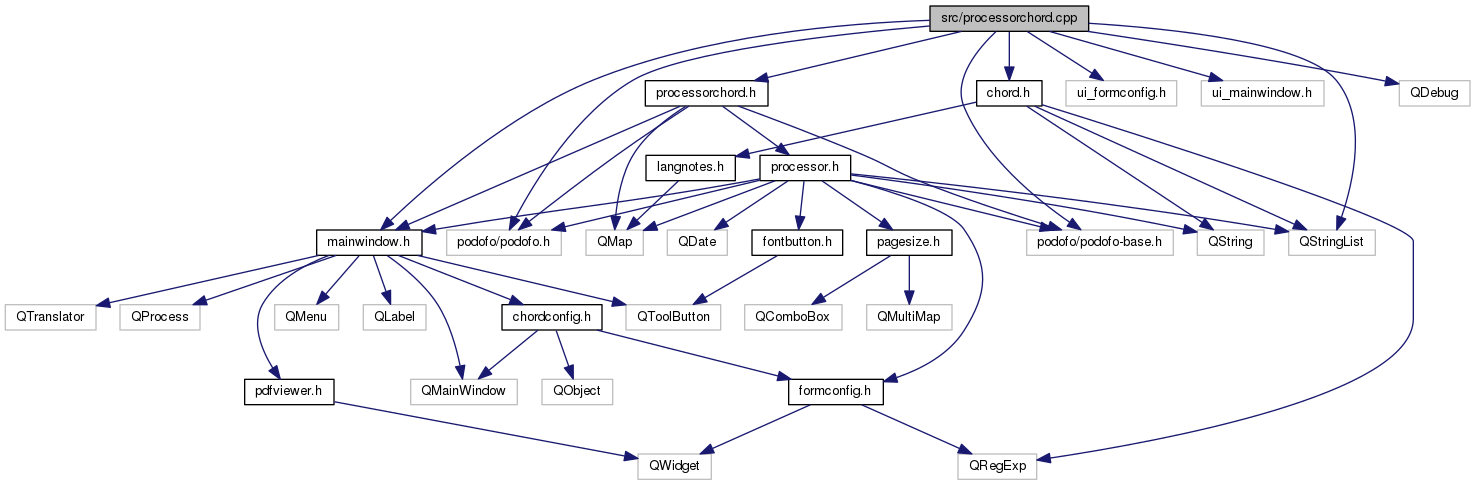
\includegraphics[width=350pt]{processorchord_8cpp__incl}
\end{center}
\end{figure}
